\documentclass[12pt]{article}

% --- Paquetes Básicos ---
\usepackage[utf8]{inputenc}
\usepackage[mexican]{babel}
\usepackage{amsmath, amssymb, amsfonts} % Para rigor matemático
\usepackage{graphicx} % Para insertar diagramas 
\usepackage{geometry}
\usepackage{hyperref}
\usepackage{titlesec}
\usepackage[table]{xcolor}
\usepackage{float}
\usepackage{tikz}
\usetikzlibrary{arrows.meta, chains, positioning, shapes.geometric}
\usepackage{minted} % Para código Python
\usepackage{csquotes}
\usepackage[backend=bibtex, style=numeric, sorting=none]{biblatex}
% \addbibresource{referencias.bib} % Descomentar y crear el archivo si se necesitan referencias

% --- Configuración de Página ---
\geometry{letterpaper, margin=2.5cm}
\titleformat{\section}{\large\bfseries}{\thesection.}{0.5em}{}

% --- Información del Documento ---
\title{Tarea 4: La Transformada de Fourier, Muestreo y \\ Procesamiento de Señales No Estacionarias}
\author{Karla Romina Juárez Torres \\ \small Análisis Matemático Aplicado}
\date{318013712}

\begin{document}

\maketitle

\section*{1. Teoría Analítica: La Transformada Continua}
\subsection*{Ejercicio 1. El Teorema de la Convolución}

Demuestre formalmente que la Transformada de Fourier de la convolución de dos funciones, $f(t)$ y $g(t)$, es igual al producto de sus transformadas individuales. Es decir, demuestre que:

\begin{equation}
\mathcal{F}\{(f * g)(t)\} = F(\omega) \cdot G(\omega)
\end{equation}

\textit{Pista: Utilice la definición de la integral de convolución y realice un cambio de variable en la integral doble resultante, justificando la inversión del orden de integración mediante el Teorema de Fubini.}

\vspace{0.5cm}

\textbf{Demostración:}

Partiendo directamente de la definición analítica de la Transformada de Fourier, obtenemos la siguiente expresión:

\begin{equation}
    \mathcal{F}\{(f * g)(t)\} = \int_{-\infty}^{\infty} (f * g)(t) e^{-i\omega t} \, dt
\end{equation}

Expandiendo el término de la convolución utilizando su propia definición integral, esto es, $(f * g)(t) = \int_{-\infty}^{\infty} f(\tau) g(t - \tau) \, d\tau$ y al sustituir esta relación en nuestra ecuación original queda la siguiente integral doble

\begin{equation}
    \mathcal{F}\{(f * g)(t)\} = \int_{-\infty}^{\infty} \left( \int_{-\infty}^{\infty} f(\tau) g(t - \tau) \, d\tau \right) e^{-i\omega t} \, dt
\end{equation}

Considerando que tanto $f$ como $g$ pertenecen al espacio de funciones absolutamente integrables, podemos garantizar que la función conjunta es integrable sobre $\mathbb{R}^2$ y con esto invocar el Teorema de Fubini así se invierte el orden de integración

\begin{equation}
    \mathcal{F}\{(f * g)(t)\} = \int_{-\infty}^{\infty} f(\tau) \left( \int_{-\infty}^{\infty} g(t - \tau) e^{-i\omega t} \, dt \right) \, d\tau
\end{equation}

Si definimos $u = t - \tau$ tenempos $dt = du$ y como los límites de integración abarcan toda la recta real estos terminan permaneciendo invariantes bajo la traslación, ahora sustituyendo $t = u + \tau$ en el exponente complejo, obtenemos

\begin{equation}
    \mathcal{F}\{(f * g)(t)\} = \int_{-\infty}^{\infty} f(\tau) \left( \int_{-\infty}^{\infty} g(u) e^{-i\omega (u + \tau)} \, du \right) \, d\tau
\end{equation}

Ahora si factorizamos el término $e^{-i\omega (u + \tau)}$ como el producto $e^{-i\omega u} e^{-i\omega \tau}$ y dado que $e^{-i\omega \tau}$ es completamente independiente de $u$ queda

\begin{equation}
    \mathcal{F}\{(f * g)(t)\} = \int_{-\infty}^{\infty} f(\tau) e^{-i\omega \tau} \left( \int_{-\infty}^{\infty} g(u) e^{-i\omega u} \, du \right) \, d\tau
\end{equation}
Notesé que la integral interna entre paréntesis corresponde de manera exacta a la definición de la Transformada de Fourier de la función $g(t)$ si llamamos a esto $G(\omega)$ y como esto ya no depende de la variable de integración externa $\tau$, funge como una constante que multiplica a la integral restante entonces tenemos

\begin{equation}
    \mathcal{F}\{(f * g)(t)\} = G(\omega) \int_{-\infty}^{\infty} f(\tau) e^{-i\omega \tau} \, d\tau
\end{equation}

Entonces la integral que sobrevive es la Transformada de Fourier de la función $f(t)$ osea $F(\omega)$, por lo que, al sustituir este último término tenemos

\begin{equation}
    \mathcal{F}\{(f * g)(t)\} = G(\omega) \cdot F(\omega) = F(\omega) \cdot G(\omega)
\end{equation}

De esta manera se confirma que la convolución en el dominio del tiempo es equivalente a la multiplicación en el dominio de la frecuencia. \hfill $\blacksquare$

\subsection*{Ejercicio 2. Cálculo de Integral Directa}

Calcule la Transformada de Fourier de la función pulso rectangular unitario $\Pi(t)$, definida como $1$ para $|t| < 1/2$ y $0$ en otro caso. Exprese el resultado en términos de la función $\operatorname{sinc}(x) = \frac{\sin(\pi x)}{\pi x}$.

\vspace{0.5cm}

\textbf{Desarrollo:}

Recordando que esta transformación mapea una señal del dominio temporal al dominio de las frecuencias angulares partimos de
\begin{equation}
    \mathcal{F}\{f(t)\} = \int_{-\infty}^{\infty} f(t) e^{-i\omega t} \, dt
\end{equation}

Ahora considerando la definición seccionalmente continua de $\Pi(t)$ que toma el valor de uno exclusivamente en el intervalo abierto de $-1/2 < t < 1/2$ y se anula en cualquier otro instante la integral colapsa a una integral definida sobre este soporte acotado

\begin{equation}
    \mathcal{F}\{\Pi(t)\} = \int_{-1/2}^{1/2} (1) e^{-i\omega t} \, dt
\end{equation}

Al integrar tenemo

\begin{equation}
    \mathcal{F}\{\Pi(t)\} = \left[ \frac{e^{-i\omega t}}{-i\omega} \right]_{-1/2}^{1/2}
\end{equation}

Ahora si evaluamos en los límites de integración:

\begin{equation}
    \mathcal{F}\{\Pi(t)\} = \frac{e^{-i\omega(1/2)} - e^{-i\omega(-1/2)}}{-i\omega} = \frac{e^{-i\omega/2} - e^{i\omega/2}}{-i\omega}
\end{equation}

Multiplicamos por $-1$ en numerador y denominador para reordenar los términos del numerador tenemos

\begin{equation}
    \mathcal{F}\{\Pi(t)\} = \frac{e^{i\omega/2} - e^{-i\omega/2}}{i\omega}
\end{equation}

Ahora la estructura de la ecuación indica la aplicación de la identidad de Euler para la función seno que dice que $\sin(\theta) = \frac{e^{i\theta} - e^{-i\theta}}{2i}$ y al proyectar esta identidad sobre nuestra expresión con el argumento $\theta = \omega/2$ la ecuación se transforma en

\begin{equation}
    \mathcal{F}\{\Pi(t)\} = \frac{2i \sin(\omega/2)}{i\omega} = \frac{2 \sin(\omega/2)}{\omega}
\end{equation}

Esta última forma se muestra la naturaleza oscilatoria y decreciente del espectro y si reacomodamos el factor $2$ en el denominador obtenemos

\begin{equation}
    \mathcal{F}\{\Pi(t)\} = \frac{\sin(\omega/2)}{\omega/2}
\end{equation}

Ahora esto nos exige expresar este resultado en términos de la función seno cardinal normalizada y para acatar esta convención, proponemos un argumento $x$ tal que garantice la equivalencia $\pi x = \omega / 2$ y por lo tanto tenemos que $x = \frac{\omega}{2\pi}$ y al insertar este cambio de variable obtenemos que

\begin{equation}
    \mathcal{F}\{\Pi(t)\} = \frac{\sin\left(\pi \left(\frac{\omega}{2\pi}\right)\right)}{\pi \left(\frac{\omega}{2\pi}\right)} = \operatorname{sinc}\left(\frac{\omega}{2\pi}\right)
\end{equation}

Entonces la Transformada de Fourier del pulso rectangular en el dominio del tiempo se manifiesta como una función seno cardinal normalizada en el dominio de la frecuencia

\begin{equation}
    \mathcal{F}\{\Pi(t)\} = \operatorname{sinc}\left(\frac{\omega}{2\pi}\right)
\end{equation}


\section*{2. Procesamiento Digital de Señales (DSP)}
\subsection*{Ejercicio 3. El Límite de Nyquist y el Aliasing}

Defina y explique con sus propias palabras:

\begin{enumerate}
    \item \textbf{Frecuencia de Nyquist:} ¿Cuál es la relación mínima necesaria entre la frecuencia de muestreo ($f_s$) y la frecuencia máxima de la señal ($f_{\text{max}}$)?
    \item \textbf{Aliasing:} Explique matemáticamente el fenómeno de ``solapamiento'' que ocurre cuando se viola el teorema de muestreo. ¿Cómo se ve reflejado en el espectro de potencias?
    \item \textbf{Ventaneo (Windowing):} En señales finitas, la FFT asume periodicidad. Explique para qué sirven funciones como Hamming o Hanning y cómo mitigan el fenómeno de ``Spectral Leakage''.
\end{enumerate}

\vspace{0.5cm}

\textbf{Definiciones Analíticas:}

\begin{enumerate}
    \item Frecuencia de Nyquist: En el procesamiento digital de señales tenemos que la fidelidad de la información depende de la tasa de adquisición de datos, es decir, del número de muestras que se toman por segundo entonces el Teorema de Muestreo de Nyquist-Shannon impone una restricción para reconstruir una señal analógica a partir de un conjunto discreto de muestras sin que se sufran perdidas ni alteraciones de la información original, es necesario que la frecuencia de muestreo $f_s$ sobrepase el doble de la componente espectral más alta $f_{\text{max}}$ presente en dicha señal, es decir $f_s > 2 f_{\text{max}}$, y entocnes el umbral $f_N = f_s / 2$ es conocido como la Frecuencia de Nyquist la cual dicta el límite superior o frontera de frecuencias que el sistema es capaz de resolver.
    
    \item Aliasing: Cuando la restricción de Nyquist es violada es decir $f_s \leq 2 f_{\text{max}}$ sucede un fenómeno de distorsión que llamamos aliasing o solapamiento donde el acto de muestrear una función equivale a modularla, es decir, multiplicarla por una infinita suma de deltas de Dirac y por el teorema de convolución que demostramos en el primer inciso esta multiplicación temporal queda como una convolución en el dominio de la frecuencia la cual genera infinitas réplicas del espectro original desplazadas cada $f_s$ hercios. 
    
    Mientras se respete el criterio de Nyquist, estas copias espectrales coexisten de manera separada y ortogonal, sin embargo al tener una tasa de muestreo deficiente el espaciamiento $f_s$ resulta insuficiente para albergar la anchura total del espectro y dado que las bandas se intersectan las colas de frecuencias altas de una réplica se suman a las frecuencias bajas de la réplica adyacente. 
    
    Esta interferencia constructiva se manifiesta como frecuencias fantasma con componentes de alta energía que superan el límite de Nyquist, que rebotan hacia la región observable y terminan camuflándose como armónicos de baja frecuencia que termina corrompiendo la lectura del periodograma.
    
    \item Ventaneo (Windowing): Al emplear algoritmos numéricos como la Transformada Rápida de Fourier (FFT), se asume que el fragmento de la señal discreta constituye un período de una señal que se repite de forma infinita. En la practica experimental al aislar un bloque de tiempo de una señal continua se tendria que es estadísticamente improbable que los valores de amplitud en los extremos inicial y final coincidan perfectamente. Asú al concatenar este bloque para cumplir con la periodicidad se terminan forzando discontinuidades o saltos abruptos en las fronteras
    
    Si consideramos que cualquier cambio súbito en el dominio del tiempo requiere de altas frecuencias para ser sintetizado, estas discontinuidades artificiales terminan inyectando energía al espectro lo que provoca que la potencia real de las componentes frecuenciales se derrame hacia los canales adyacentes que es un efecto perjudicial tipificado como \textit{Spectral Leakage} entonces para mitigar esta anomalía numérica aplicamos funciones de ventana como las de Hamming o Hanning que consisten en perfiles de ponderación suave que alcanzan su máximo en el centro del bloque y decaen asintóticamente a cero en los extremos asi al multiplicar la señal por dicha ventana logramos una transición periódica suave que atenúa los lóbulos laterales del espectro y purifica la lectura frecuencial.
\end{enumerate}

\subsection*{Ejercicio 4. Estructura de la DFT y FFT}

Analice el siguiente diagrama de flujo que representa la lógica de cómputo para transformar una señal del dominio del tiempo al de la frecuencia.

\begin{figure}[H]
    \centering
    \begin{tikzpicture}[
        node distance=2cm and 1cm,
        box/.style={draw, rectangle, align=center, minimum width=3cm, minimum height=1cm},
        arrow/.style={-Latex, thick}
    ]
        % Nodes
        \node[box] (signal) {Señal Discreta $x[n]$};
        \node[box, below left=of signal] (dft) {DFT Directa ($\mathcal{O}(N^2)$)};
        \node[box, below right=of signal] (fft) {FFT (Cooley-Tukey)\\($\mathcal{O}(N \log N)$)};
        \node[box, below=3cm of signal] (espectro) {Espectro $X[k]$};

        % Arrows and Labels
        \draw[arrow] (signal) -| (dft) node[pos=0.25, left, align=right] {Muestreo a $f_s$\\Condición: $f_s > 2f_{\text{max}}$};
        \draw[arrow] (signal) -| (fft);
        \draw[arrow] (dft) |- (espectro);
        \draw[arrow] (fft) |- (espectro);
    \end{tikzpicture}
    \caption{Diagrama de flujo de la transformación de señales.}
    \label{fig:diagrama_fft}
\end{figure}

\vspace{0.5cm}

\textbf{Análisis de Flujo y Complejidad:}

El proceso inicia en la etapa de muestreo, donde el diagrama resalta la necesidad de cumplir con el criterio de Nyquist como necesitamos eso para poder digitalizar una señal analógicay esto funciona para evitar el antialiasing antes de aplicar cualquier transformación

Una vez que se dispone de la secuencia digital $x[n]$, el flujo se divide en dos procesos, sin embargo, convergen en el mismo resultado esto nos deja claro que la Transformada Rápida de Fourier no es una aproximación numérica sino una ruta matemáticamente idéntica a la Transformada Discreta de Fourier.

La diferencia entre ambos procesos radica en el costo computacional:
\begin{itemize}
    \item La DFT Directa sigue la definición matemática formal mediante la sumatoria:
    \begin{equation*}
    X[k] = \sum_{n=0}^{N-1} x[n] e^{-i \frac{2\pi}{N} k n}
    \end{equation*}
    Al implementarse a fuerza bruta, obliga al sistema a realizar un número de multiplicaciones complejas proporcional al cuadrado del número de muestras, lo que genera una complejidad algorítmica de orden $\mathcal{O}(N^2)$. Con los enormes volúmenes de datos, este crecimiento cuadrático se vuelve rápidamente inviable en la práctica.
    
    \item La FFT de Cooley-Tukey tiene la estrategia de ``divide y vencerás'' para aprovechar las propiedades de simetría y periodicidad de las exponenciales complejas como los conocidos \textit{twiddle factors} o factores de giro para dividir la señal original en transformaciones mucho más pequeñas por ejemplo, separando las muestras pares de las impares, lo que reduce drásticamente las operaciones necesarias y termina colapsando la complejidad a $\mathcal{O}(N \log_2 N)$.
\end{itemize}


\section*{3. Laboratorio: Señales No Estacionarias}
\subsection*{Ejercicio 5. Programación y Filtrado}

Una señal no estacionaria es aquella cuyas propiedades estadísticas (frecuencia, amplitud) varían con el tiempo. Para estas señales, una sola FFT ``promedia'' todo el tiempo y pierde la información de cuándo ocurrieron los eventos.

Programe en Python las siguientes funciones en un dominio de 2 segundos ($f_s = 1000$ Hz):
\begin{enumerate}
    \item \textbf{Señal A (Chirp):} $s_1(t) = \sin(2\pi(10 + 40t)t)$. (Frecuencia que sube de 10 a 90 Hz).
    \item \textbf{Señal B (Salto de Frecuencia):} $s_2(t) = \sin(2\pi 20t)$ para $t < 1\text{s}$, y $s_2(t) = \sin(2\pi 80t)$ para $t \geq 1\text{s}$.
\end{enumerate}

\textbf{Requerimientos del Código:}
\begin{itemize}
    \item Calcule y grafique la FFT de ambas señales. Observe cómo en la Señal B aparecen dos picos, pero se pierde la noción de qué frecuencia va primero.
    \item Aplique un filtro pasa-altas con corte en 50 Hz a ambas señales en el dominio de la frecuencia.
    \item Realice la IFFT y grafique el resultado en el tiempo. Describa qué sucede con la parte inicial de la Señal B tras el filtrado.
\end{itemize}

\vspace{0.5cm}

\textbf{Solución:}


En primera instancia se calculan y grafican las transformadas de Fourier de ambas señales para poder observar el espectro de frecuencias y como este se distribuye en el dominio de la frecuencia. Si observamos la Señal B, se aprecian con total claridad dos picos dominantes en las frecuencias de $20\text{ Hz}$ y $80\text{ Hz}$, sin embargo, como la transformada de Fourier integra la señal a lo largo de todo el intervalo y la magnitud del espectro termina actuando como un promedio de todas las oscilaciones. Entonces aunque el espectro nos dice que frecuencias están presentes pierde la información de cuando aparecieron donde si miramos la gráfica de magnitud, es imposible saber si el pulso de $20\text{ Hz}$ ocurrió antes que el de $80\text{ Hz}$, si fue al revés, o si ambos tonos sonaron al mismo tiempo durante toda la simulación.

Por otra parte, el filtrado de la señal en el dominio de la frecuencia ofrece resultados muy predecibles y consistentes con la teoría esto es por que aplica un filtro pasa-altas ideal con una frecuencia de corte estricta en $50\text{ Hz}$ así se elimina cualquier componente espectral por debajo de ese límite y como el primer segundo de la Señal B consistía únicamente en un tono puro de $20\text{ Hz}$, esta primera mitad de la señal es eliminada por completo por el filtro.

Como consecuencia al aplicar la Transformada Inversa para regresar la señal manipulada al dominio del tiempo notamos cómo la primera mitad del vector prácticamente desaparece. La amplitud entre $t=0$ y $t=1\text{ s}$ es casi cero, mostrando un decaimiento, mientras que a partir de $t=1\text{ s}$ la señal de $80\text{ Hz}$ se mantiene intacta tras haber superado el corte del filtro. 

Cabe mencionar que justo en la discontinuidad de $t=1\text{ s}$ aparecen unas pequeñas oscilaciones que se deben al fenómeno de Gibbs que surge al multiplicar el espectro por una función escalón rectangular, la cual requeriría un ancho de banda infinito para recrear un cambio tan abrupto en el tiempo de forma perfecta.

\begin{minted}[bgcolor=lightgray!20, fontsize=\small, linenos]{python}
import numpy as np
import matplotlib.pyplot as plt
from numpy.fft import fft, ifft, fftfreq

# Parámetros
fs = 1000
T = 2.0
t = np.linspace(0, T, int(fs * T), endpoint=False)
N = len(t)

# Señal A (Chirp): s1(t) = sin(2*pi*(10 + 40t)*t)
s1 = np.sin(2 * np.pi * (10 + 40 * t) * t)

# Señal B (Salto de Frecuencia): 
# s2(t) = sin(2*pi*20*t) para t < 1, y sin(2*pi*80*t) para t >= 1
s2 = np.piecewise(t, [t < 1, t >= 1], [
    lambda t: np.sin(2 * np.pi * 20 * t), 
    lambda t: np.sin(2 * np.pi * 80 * t)
])

# Transformada de Fourier
S1 = fft(s1)
S2 = fft(s2)
freqs = fftfreq(N, 1/fs)

# Filtro Pasa-Altas
cutoff = 50
high_pass_filter = np.abs(freqs) >= cutoff

# Aplica el filtro en el dominio de la frecuencia
S1_filtered = S1 * high_pass_filter
S2_filtered = S2 * high_pass_filter

# Aplica la Transformada Inversa para obtener señales filtradas en el tiempo
s1_filtered = np.real(ifft(S1_filtered))
s2_filtered = np.real(ifft(S2_filtered))
\end{minted}

\begin{figure}[H]
    \centering
    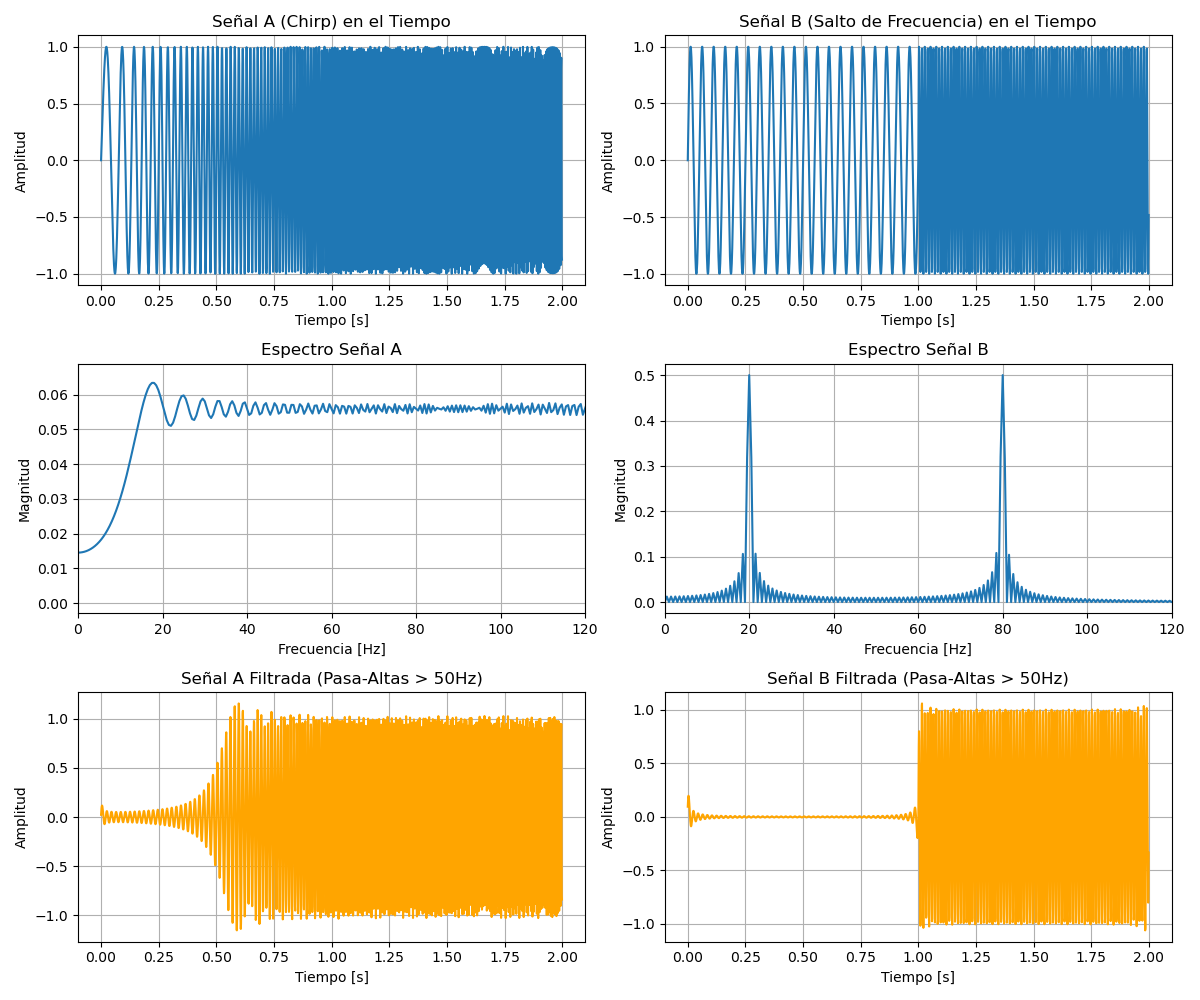
\includegraphics[width=\textwidth]{ejercicio5_grafica.png}
    \caption{Señales en el tiempo, sus respectivos espectros de frecuencia y el resultado tras aplicar un filtro pasa-altas con corte en 50 Hz.}
    \label{fig:ejercicio5}
\end{figure}


% \newpage
% \printbibliography[title={Bibliografía}]

\end{document}
